\documentclass[twoside,11pt,a4paper]{article}
\usepackage{style/jmlr2e,amsfonts,amsmath,tikz,hyperref,microtype,pgfplots,graphicx}
\usetikzlibrary{patterns,arrows,calc,positioning} 

\jmlrheading{}{}{}{}{}{Lopez-Paz, Muandet and Recht}
\ShortHeadings{The Randomized Causation Coefficient}{Lopez-Paz, Muandet and Recht}

\definecolor{mydarkblue}{rgb}{0,0.08,0.45}

\hypersetup{
  colorlinks = true,
  linkcolor  = mydarkblue,
  citecolor  = mydarkblue,
  filecolor  = mydarkblue, 
  urlcolor   = mydarkblue
} 

\newcommand\ci{\perp\!\!\!\perp}

\newcommand{\KM}[1]{\textcolor{blue}{[ KM: #1 ]}}
\newcommand{\DLP}[1]{\textcolor{red}{[ DLP: #1 ]}} 
\DeclareMathOperator*{\argmin}{arg\,min}
\DeclareMathOperator*{\argmax}{arg\,max}

\newcommand{\U}{\mathcal{U}}
\newcommand{\N}{\mathcal{N}} 
\renewcommand{\P}{\mathcal{P}}

\begin{document} 

\title{The Randomized Causation Coefficient}

\author{\name David Lopez-Paz\thanks{This project was conceived while DLP was
visiting BR at University of California, Berkeley.} \email david@lopezpaz.org
\\
        \addr Max Planck Institute for Intelligent Systems\\
        \addr University of Cambridge\\
        \name Krikamol Muandet \email krikamol@tuebingen.mpg.de \\
        \addr Max Planck Institute for Intelligent Systems\\
        \name Benjamin Recht  \email brecht@berkeley.edu\\
        \addr University of California, Berkeley\\
}

\editor{TBD}
\maketitle 

\begin{abstract}%
  We are interested in learning causal relationships between pairs of random
  variables, purely from observational data. To effectively address this task,
  the state-of-the-art relies on strong assumptions on the mechanisms
  mapping causes to effects, such as invertibility or the existence of additive
  noise, which only hold in limited situations.
  %
  On the contrary, this short paper proposes to \emph{learn} how to perform
  causal inference directly from data, without the need of feature
  engineering. In particular, we pose causality as a kernel mean embedding
  classification problem, where inputs are samples from arbitrary probability
  distributions on pairs of random variables, and labels are types of causal
  relationships.
  %
  We validate the performance of our method on synthetic and real-world data
  against the state-of-the-art. Moreover, we submitted our algorithm to the
  ChaLearn's ``Fast Causation Coefficient Challenge'' competition, with which
  we won the fastest code prize and ranked third in the overall leaderboard.
\end{abstract}

\section{Introduction}\label{sec:intro}
According to Reichenbach's common cause principle \citep{Reichenbach56:Time},
the dependence between two random variables $X$ and $Y$ implies that either $X$
causes $Y$ (denoted by $X \rightarrow Y$), or that $Y$ causes $X$ (denoted by
$Y \rightarrow X$), or that $X$ and $Y$ have a common cause. In this note, we
are interested in distinguishing between these three possibilities by using
samples drawn from the joint probability distribution $P$ on $(X,Y)$.

Two of the most successful approaches to tackle this problem are the
information geometric causal inference method \citep{Daniusis12,Janzing14}, and
the additive noise model~\citep{Hoyer09,Peters14:ANM}. 
%
First, the Information Geometric Causal Inference (IGCI) is designed to infer
causal relationships between variables related by invertible, noiseless
relationships.  In particular, assume that there exists a pair of functions or
\emph{mapping mechanisms} $f$ and $g$ such that $Y = f(X)$ and $X = g(Y)$. The
IGCI method decides that $X \rightarrow Y$ if $\rho(P(X),|\log(f'(X))|)< 
\rho(P(Y),|\log(g'(Y))|)$, where $\rho$ denotes Pearson's correlation coefficient.
IGCI decides $Y \rightarrow X$ if the opposite inequality holds, and abstains
otherwise.  The assumption here is that the cause random variable is
independently generated from the mapping mechanism; therefore it is unlikely to
find correlations between the density of the former and the slope of the latter. 
%
Second, the additive noise model (ANM) assumes that the effect variable is
equal to a nonlinear transformation of the cause variable plus some independent
random noise, i.e., $Y = f(X) + N_Y$. If $X\ci N_Y$,
then there exists no model of the form $X = g(Y) + N_X$ for which
$Y\ci N_X$. As a result, one can find the causal direction by
performing independence test between the input variable and residual
variable in both directions. Specifically,
the algorithm will conclude that $X \rightarrow Y$ if the pair of random variables
$(X, N_Y)$ are independent but the pair $(Y, N_X)$ is not. The algorithm will
conclude $Y \rightarrow X$ if the opposite claim is true, and abstain
otherwise. The additive noise model has been extended to study post-nonlinear
models of the form $Y = h(f(X)+N_Y)$, where $h$ a monotone function
\citep{Zhang09}. The consistency of causal inference under the additive noise
model was established by \citet{Kpotufe13} under some technical assumptions.

As it becomes apparent from the previous exposition, there is a lack of a
general method to infer causality without assuming strong knowledge about the
underlying causal mechanism.  Moreover, it is desirable to readily extend
inference to other new model hypotheses without incurring in the development of
a new, specific algorithm. Motivated by this issue, we raise the question,

\begin{center}
  \emph{Is it possible to automatically learn patterns revealing causal
  relationships between random variables from large amounts of labeled data?}
\end{center}

\section{Learning to Learn Causal Inference} 

Unlike the methods described above, we propose a \emph{data-driven approach} to
build a flexible causal inference engine.  To do so, we assume access to some
set of pairs $\{(S_i,l_i)\}_{i=1}^n$, where the sample $S_i
=\{(x_{ij},y_{ij})\}_{j=1}^{n_i}$ are drawn i.i.d. from the joint distribution
$P_i$ of the two random variables $X_i$ and $Y_i$, which obey the causal
relationship denoted by the label $l_i$.  To simplify exposition, the labels
$l_i = 1$ denotes $X \rightarrow Y$ and $l_i = -1$ stands for $Y \rightarrow
X$.  Using these data, we build a causal inference algorithm in two steps.
First, an $m$-dimensional feature vector $\mathbf{m}_i$ is extracted from each
sample $S_i$, to meaningfully represent the corresponding distribution $P_i$.
Second, we use the set $\{(\mathbf{m}_i, l_i)\}_{i=1}^{n}$ to train a binary
classifier, later used to predict the causal relationship between previously
unseen pairs of random variables.  This framework can be straightforwardly
extended to also infer the ``common cause'' and ``independence'' cases, by
introducing two extra labels. 

Our setup is fundamentally different from the standard classification problem
in the sense that the inputs to the learners are samples from probability
distributions, rather than real-valued vectors of features
\citep{Muandet12,Szabo14}.  In particular, we place two assumptions.
First, the existence of a \emph{Mother distribution}
$\mathcal{M}(\mathcal{P},\{-1,+1\})$ from which all paired probability
distributions $P_i \in \mathcal{P}$ on $(X_i,Y_i)$ and causal labels $l_i \in
\{-1,+1\}$ are sampled, where $\mathcal{P}$ denotes the set of all distributions on
two real-valued random variables. Second, the causal relationships $l_i$ can be
inferred in most cases from observable properties of the distributions $P_i$.
While these assumptions may not hold in generality, our experimental evidence
suggests their wide applicability in real-world data.

The rest of this paper is organized as follows.  Section~\ref{sec:features}
elaborates on how to extract the $m-$dimensional feature vectors $\mathbf{m}_i$ from
each causal sample $S_i$.  Section~\ref{sec:exps} provides empirical evidence
to validate our methods. Section~\ref{sec:future} closes the
exposition by commenting on future research directions. 

\section{Featurizing Distributions with Kernel Mean Embeddings}
\label{sec:features}
Let $P$ be the probability distribution of some random variable $Z$ taking
values in $\mathbb{R}^d$.  Then, the \emph{kernel mean embedding} of $P$
associated with the positive definite kernel function $k$ is 
\begin{equation}
  \label{eq:meank}
  \mu_k(P) := \int_{\mathbb{R}^d} k(z, \cdot) \mathrm{d}P(z) \in
  \mathcal{H}_k,
\end{equation}
where $\mathcal{H}_k$ is the reproducing kernel Hilbert space (RKHS) endowed
with the kernel $k$ \citep{Berlinet04:RKHS,Smola07Hilbert}. A sufficient
condition which guarantees the existence of $\mu_k$ is that the kernel $k$ is
bounded, i.e., $\sup_{z\in\mathcal{Z}}k(z,z) < \infty$. One of the most
attractive property of $\mu_k$ is that it uniquely determines each distribution
$P$ when $k$ is a characteristic kernel \citep{Sriperumbudur10:Metrics}. In
another words,
$\|\mu_k(P)-\mu_k(Q)\|_{\mathcal{H}_k}=0$ iff $P=Q$. Examples of characteristic
kernels include the popular squared-exponential
\begin{equation}\label{eq:gauss}
  k(z,z') = \exp\left(-\gamma \|z- z'\|_2^2\right), \text{ for }
  \gamma >0,
\end{equation}
which will be used throughout this work.

However, in practice, we do not have access to the true
distribution $P$, and consequently to the true embedding $\mu_k$. Instead, we
often have access to a sample $S = \{z_i\}_{i=1}^n$
drawn i.i.d.  from $P$. Then, we can construct the empirical measure $P_S =
\frac{1}{n} \sum_{i=1}^n \delta_{(z_i)}$, where $\delta_{(z)}$ is the Dirac
mass at $z$, and estimate \eqref{eq:meank} by 
\begin{equation}
  \label{eq:meank2} 
  {\mu}_k(P_S) := \frac{1}{n} \sum_{i=1}^n k(z_i, \cdot) \in \mathcal{H}_k.
\end{equation}
Though it can be improved \citep{Muandet14:KMSE}, the estimator
\eqref{eq:meank2} is the most common due to its ease of implementation. We can
essentially view \eqref{eq:meank} and \eqref{eq:meank2} as the feature
representations of the distribution $P$ and its sample $S$, respectively. 

For some kernels such as \eqref{eq:gauss}, the feature maps \eqref{eq:meank}
and \eqref{eq:meank2} do not have a closed form, or are infinite dimensional.
This translates into the need of kernel matrices, which require at least
$O(n^2)$ computation. In order to alleviate these burdens, we propose to
compute a low-dimensional approximation of \eqref{eq:meank2} using random
Fourier features \citep{Rahimi07}. In particular, if the kernel $k$ is
shift-invariant, we can exploit Bochner's theorem \citep{Rudin62} to construct
a randomized approximation of \eqref{eq:meank2}, with form
\begin{equation}\label{eq:meank3}
  {\mu}_{k,m}(P_S) = \frac{1}{n} \sum_{i=1}^n \left[ \cos(w_1'
  z_i + b_1), \ldots, \cos(w_m' z_i + b_m)\right]' \in
  \mathbb{R}^m,
\end{equation}
where the vectors $w_1, \ldots, w_m \in \mathbb{R}^d$ are sampled from the normalized Fourier
transform of $k$, and $b_1, \ldots, b_m \sim \mathcal{U}(0, 2\pi)$. The
squared-exponential kernel in \eqref{eq:gauss} is shift-invariant, and can be
approximated in this fashion when setting $w_i \sim \mathcal{N}(0,
2\gamma I)$.  These features can be computed in $O(mn)$ time and stored in
$O(1)$ memory. Importantly, the low dimensional representation
${\mu}_{k,m}$ is amenable for the off-the-shelf use with any standard
learning algorithm, and not only kernel-based methods.

Using the assumptions introduced in Section~\ref{sec:intro}, the data
$\{(\mathbf{m}_i,l_i)\}_{i=1}^n := \{(\mu_{k,m}(P_{S_i}),l_i)\}_{i=1}^n$ and a binary
classifier, we can now pose causal inference as a supervised learning problem.

\section{Numerical Simulations}\label{sec:exps}
We conduct an array of experiments to test the effectiveness of a simple
implementation of the presented causal learning framework\footnote{Source code
available at
{\small\url{https://github.com/lopezpaz/causation_learning_theory}}}. Given the
use of random embeddings \eqref{eq:meank3} in our classifier, we term our
method the \emph{Randomized Causation Coefficient} (RCC).  Throughout our
simulations, we featurize each sample $S = \{(x_{i},y_{i})\}_{i=1}^{n}$ as
\begin{align}\label{eq:ourfeatz}
  \nu(S) = (\mu_{k,m}(P_{S_x}), \mu_{k,m}(P_{S_y}), \mu_{k,m}(P_{S})),
\end{align}
where the three elements forming \eqref{eq:ourfeatz} stand for the
low-dimensional representations \eqref{eq:meank3} of the empirical kernel mean
embeddings of $\{x_i\}_{i=1}^n$, $\{y_i\}_{i=1}^n$, and
$\{(x_i,y_i)\}_{i=1}^n$, respectively. This representation is motivated by the
typical conjecture in causal inference about the existence of asymmetries
between the marginal and conditional distributions of causally-related pairs of
random variables \citep{Scholkopf12:Causal}. Each of these three embeddings has
random features sampled to approximate the sum of three Gaussian kernels
\eqref{eq:gauss} with hyper-parameters $0.1\gamma$, $\gamma$, and $10\gamma$,
where $\gamma$ is set using the median heuristic.  In practice, we set $m =
1000$, and observe no significant improvements when using larger amounts of
random features. To classify the embeddings \eqref{eq:ourfeatz} in each of the
experiments, we use the random forest implementation from Python's
\texttt{sklearn-0.16-git}. The number of trees forming the forest is chosen
from the set $\{100,250,500,1000,5000\}$, via cross-validation.
\subsection{T\"ubingen Data}
The \emph{T\"ubingen cause-effect pairs} is a collection of heterogeneous,
hand-collected, real-world cause-effect
samples\footnote{\url{https://webdav.tuebingen.mpg.de/cause-effect/}}. Given
the small size of this dataset, we resort to the synthesis of some Mother
distribution to sample our training data from.  To this end, assume that
sampling a synthetic cause-effect sample $\hat{S}_i := \{(\hat{x}_{ij},
\hat{y}_{ij})\}_{j=1}^n$ equals the following 
generative process:
\begin{enumerate}
  \item A \emph{cause} vector $(\hat{x}_{ij})_{j=1}^{n}$ is sampled from a
  mixture of Gaussians with $c$ components. The mixture weights are
  sampled from $\U(0,1)$, and normalized to sum to one. The mixture means and
  standard deviations are sampled from $\N(0,\sigma_1)$, and $\N(0,\sigma_2)$,
  respectively, accepting only positive standard deviations.
  The cause vector is standardized to zero mean and unit variance.
  \item A \emph{noise} vector $(\hat{\epsilon}_{ij})_{j=1}^{n}$ is sampled from a
  centered Gaussian, with variance sampled from $\U(0,\sigma_3)$.
  \item The \emph{mapping mechanism} $\hat{f}_i$ is a spline fitted
  using an uniform grid of $d_f$ elements from
  $\min((\hat{x}_{ij})_{j=1}^n)$ to $\max((\hat{x}_{ij})_{j=1}^n)$ as inputs, and 
  $d_f$ normally distributed outputs.
  \item An \emph{effect} vector is built as $(\hat{y}_{ij} :=
  \hat{f}_i(\hat{x}_{ij})+\hat{\epsilon}_{ij})_{j=1}^n$, and
  standardized to zero mean and unit variance.
  \item Return the cause-effect sample $\hat{S}_i := \{(\hat{x}_{ij},
  \hat{y}_{ij})\}_{j=1}^n$.
\end{enumerate}
To choose a $\theta = (c,\sigma_1, \sigma_2, \sigma_3, d_f)$
that best resembles the unlabeled test data, we minimize the distance between the
embeddings of $N$ synthetic pairs and the T\"{u}bingen samples 
\begin{align*}
  \argmin_\theta \sum_{i}^{} \min_{1 \leq j \leq N} \| \nu(S_i)-\nu(\hat{S}_j) \|^2_2,
\end{align*}
over $c,d_f \in \{1, \ldots, 10\}$, and $\sigma_1, \sigma_2, \sigma_3 \in
\{0, 0.5, 1, \ldots, 5\}$, where the $\hat{S}_j$ is sampled using the
generative process described above, the $S_i$ are the T\"ubingen cause-effect
pairs, and $\nu$ is as in \eqref{eq:ourfeatz}.  This strategy can be thought of
as transductive learning, since we have access to the test inputs (but not
their underlying causal relation) at the training time.  

We set $n = 1000$, and $N = 10,000$. Using the generative process described 
above, and the best found parameter vector $\theta = (3,2,2,2,5)$, we
construct the synthetic training data 
\begin{align*}
  \{&\{\nu(\{(\hat{x}_{ij}, \hat{y}_{ij})\}_{j=1}^{n}), +1)\}_{i=1}^{N},\\
  &\{\nu(\{(\hat{y}_{ij}, \hat{x}_{ij})\}_{j=1}^{n}), -1)\}_{i=1}^{N}\},
\end{align*}
where $\{(\hat{x}_{ij}, \hat{y}_{ij})\}_{j=1}^{n} = \hat{S}_i$, and train
our classifier on it.
%
Figure \ref{fig:tuebingen} plots the classification accuracy of RCC, IGCI
\citep{Daniusis12}, and ANM \citep{Mooij14} versus the fraction of decisions
that the algorithms are forced to make out of the 82 scalar T\"uebingen
cause-effect pairs. To compare these results to other lower-performing methods,
refer to \citet{Janzing12}. Overall, RCC surpasses the state-of-the-art in these
data, with a classification accuracy of $81.61\%$ when inferring the causal
directions on all pairs. The confidence of RCC is computed using the
random forest's output class probabilities.

\begin{figure}[t]
  \begin{center}
    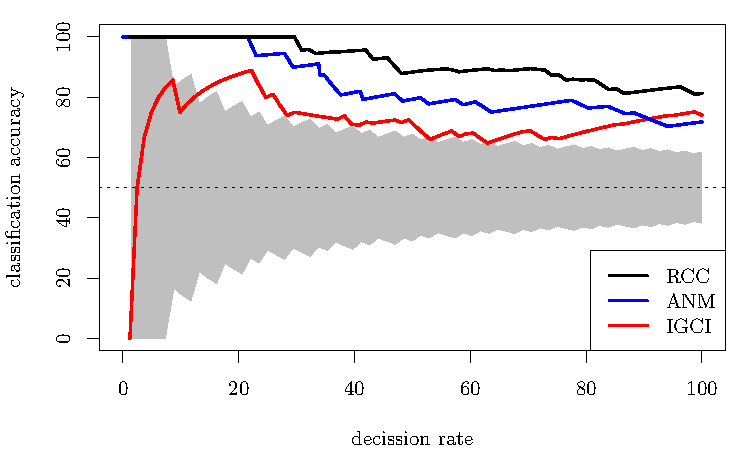
\includegraphics[width=0.8\linewidth]{plot.pdf} 
  \end{center}
  \vspace{-10pt}
  \caption{Accuracy of RCC, IGCI and ANM on the T\"ubingen cause-effect pairs,
  as a function of decision rate. The grey area depicts accuracies not
  statistically significant.}
  \label{fig:tuebingen}
\end{figure}


\subsection{ChaLearn's ``Fast Causation Coefficient'' Challenge}

We tested RCC at the ChaLearn's
\emph{Fast Causation Coefficient} challenge \citep{Codalab14}.  We trained a
Gradient Boosting Classifier (GBC), with hyper-parameters chosen via a 4-fold
cross validation, on the featurizations \eqref{eq:ourfeatz} of the training
data. In particular, we built two separate classifiers: a first one to
distinguish between causal and non-causal pairs (i.e., $X-Y$ vs $\{X\rightarrow
Y, X\leftarrow Y\}$), and a second one to distinguish between the two possible
causal directions on the causal pairs (i.e., $X\rightarrow Y$ vs $X\leftarrow
Y$). The final causation coefficient for a given sample $S_i$ was computed as
$$\mathrm{score}(S_i) = p_1(S_i)\cdot(2\cdot p_2(S_i)-1),$$ where $p_1(x)$ and
$p_2(x)$ are the class probabilities output by the first and the second GBCs,
respectively. We found it easier to distinguish between causal and non-causal
pairs than to infer the correct direction on the causal pairs.

RCC ranked third in the ChaLearn's ``Fast Causation Coefficient Challenge''
competition, and was awarded the prize to the fastest running code
\citep{Codalab14}.
%
At the time of the competition, we obtained a bidirectional AUC of $0.73$
on the test pairs in two minutes of test-time \citep{Codalab14}.
%
On the other hand, the winning entry of the competition, which made use of
hand-engineered features, took a test-time of 30 minutes, and achieved a
bidirectional AUC of $0.82$.
%
Interestingly, the performance of IGCI on the $20,000$ training pairs is barely
better than random guessing. The computational complexity of the additive noise
model (usually implemented as two Gaussian Process regressions followed by two
kernel-based independence tests) made it unfeasible to compare it on this
dataset. 

\section{Conclusions and Future Research}\label{sec:future}
To conclude, we proposed to \emph{learn how to perform causal inference} between pairs
of random variables from observational data, by posing the task as a
supervised learning problem. In particular, we introduced an effective and
efficient featurization of probability distributions, based on kernel mean
embeddings and random Fourier features. Our numerical simulations support the
conjecture that patterns revealing causal relationships can be learnt from
data.

In light of our encouraging results, we would like to mention four exciting 
research directions.  First, the proposed ideas can be used to learn other 
\emph{domain-general} statistics, such as
measures of dependence \citep{Lopez-Paz13}. Second, it is important to develop 
techniques to visualize and interpret the causal features learned by our
classifiers. This direction is particularly essential 
for causal inference as it provides a data-dependent way of discovering new 
hypothesis on underlying 
causal mechanism. Third, RCC can be extended to operate not only on pairs, 
but also sets of random variables, and eventually reconstruct causal DAGs from multivariate
data. Finally, one may adapt the distributional learning theory of
\citet{Szabo14} to analyze our randomized, classification setting. For
preliminary results on the last two points, we refer the reader to
\citep{Lopez-Paz15}.


{\small
\newpage
\bibliography{jmlr_rcc}
}
\end{document}
